\chapter{MATERIAIS E MÉTODOS}\label{ch:materiais-metodos}
Após a revisão bibliográfica de outros estudos e os fundamentos teóricos necessários para a mineração de dados utilizando Python, torna-se importante definir as ferramentas, tecnologias e procedimentos necessários para o desenvolvimento do projeto.

Este capítulo apresenta os materiais e métodos utilizados para a realização do processo de \textit{data mining}, onde, na seção~\ref{sec: tec-ferramenta} são apresentadas as tecnologias e ferramentas que serão utilizadas durante o estudo. Serão abordados quais as bibliotecas que a linguagem Python disponibiliza para a análise e mineração de dados e, também, como acessar a API do \textit{LinkedIn}. Esta será esclarecida também neste capítulo, após a explicação do conceito de API e o protocolo OAuth.

A seção~\ref{sec: metodologia} irá concluir o capítulo apresentando as etapas de \textit{data mining} com o intuito de evidenciar o processo para a obtenção de conhecimento útil.

\section{TECNOLOGIAS E FERRAMENTAS}\label{sec: tec-ferramenta}
Tecnologias e ferramentas para a criação e prototipagem dos algoritmos.

%% Bibliotecas Python
\subsection{Bibliotecas da Linguagem Python}\label{sec:bib_python}
Um dos grandes diferenciais da linguagem Python é o seu enorme conjunto de bibliotecas para soluções de diversos problemas.

A seguir serão apresentadas as bibliotecas necessárias para a mineração de dados, através das quais é possível coletar, limpar, transformar, realizar operações e apresentar resultados proveniente dos dados da rede social \textit{LinkedIn}. Para evitar repetições da palavra "biblioteca", o termo "pacote"\space também será utilizado com o mesmo significado no restante desta dissertação.
 
%%% sub: NumPy
\subsubsection{\textit{Biblioteca NumPy}}
\textit{NumPy} é o pacote fundamental para computação científica em Python. É o acrônico para \textit{Numerical Python}. Esta biblioteca provê:

\begin{itemize}
    \item \textit{ndarray} que é um objeto de matriz multidimensional;
    \item Funções que permitem realizar operações vetoriais ou operações matemáticas entre matrizes sem a necessidade de programar \textit{loops};
    \item Ferramentas para a leitura e escrita em conjuntos de dados matriciais;
    \item Operações de álgebra linear, transformada de Fourier e geração de números aleatórios;
    \item Ferramentas para a integração em outras linguagens de programação como C, C++ e Fortran.
\end{itemize}

Além da capacidade de rápido processamento em matrizes que o \textit{NumPy} oferece ao Python, um dos principais objetivos em relação a análise de dados é que serve como um "container"\space para os dados serem passado por algoritmos. Para dados numéricos, as matrizes de \textit{NumPy} são muito mais eficientes para a ordenação e manipulação de dados do que qualquer outra estrutura embutida em Python. Igualmente, bibliotecas escritas em linguagens de baixo nível, como C ou Fortran, podem operar dados gravados em matrizes da \textit{NumPy} sem precisar da cópia de qualquer dado \cite{python-analysis}.

A biblioteca \textit{NumPy} por si só, não provê uma funcionalidade de alto-nível para a análise de dados. Tendo um conhecimento sobre as matrizes de \textit{NumPy} e matrizes orientadas a computação (\textit{array-oriented computing}) irá facilitar o uso de outras ferramentas, como \textit{pandas}, com mais efetividade.

Para aplicações voltadas para a análise de dados, esta biblioteca possui grande funcionalidade em setores como:

\begin{itemize}
    \item Criação rápida de matrizes para a interação e limpeza de dados, separação e filtragem, transformação e outros tipos de operações computacionais;
    \item Algoritmos comuns para matrizes como ordenação, operações únicas e definidas;
    \item Eficiente descrição estatística e agregação/sumarização de dados;
    \item Alinhamento de dados e manipulação de dados relacionais para operações de junção e imerção (\textit{join} e \textit{merge}) de conjuntos de dados heterogeneos;
    \item Expressar lógicas de condições através de expressões matriciais ao invés de laços de repetições e condições como \textit{while, for, if-elif-else};
    \item Agrupamento de manipulação de dados (agregação, transformação, aplicação de funções).
\end{itemize}

Enquanto \textit{NumPy} oferece o fundamento computacional para essas operações, é preferível utilizar a biblioteca \textit{pandas} como base para a mineração de dados (especialmente de dados estruturados ou dados tabulados), devido a sua interface rica e de alto-nível no qual permite as tarefas com dados mais concisas e simples.

%%% sub: pandas
\subsubsection{Biblioteca \textit{pandas}}
A biblioteca \textit{pandas} atrai o maior interesse de cientistas quanto a mineração de dados. Ela possui estruturas de dados de alto-nível e ferramentas de manipulação desenvolvidas para facilitar e agilizar a análise de dados em Python. \textit{pandas} é desenvolvida sob a biblioteca \textit{NumPy} e viabiliza o uso em aplicações centradas nesta. A seguir são expostas algumas soluções que a biblioteca disponibiliza \cite{python-analysis}:

\begin{itemize}
    \item Estrutura de dados com eixos rotulados suportam o alinhamento de dados automáticos ou explícitos. Isso evita erros comuns resultantes de dados desalinhados e dados indexados de formas diferentes provenientes de outras fontes de dados;
    \item A mesma estrutura de dados consegue manusear tanto dados de séries temporais como dados não-temporais;
    \item Operações e reduções aritméticas é passado para metadados (eixos rotulados);
    \item Manipulação flexível de dados em falta;
    \item \textit{Merge} (fundir) e outras operações relacionais encontradas em bancos de dados relacional.
\end{itemize}

Esta biblioteca possui duas estrutura de dados principais: \textit{Series} e \textit{DataFrame}. Estas estruturas não são uma solução universal para todos os problemas, mas provê uma base sólida e de fácil manipulação para a maioria das aplicações com mineração de dados.

Uma \textit{Series} é um tipo de \textit{array} ou uma matriz unidimensional, similar a um \textit{array} que possui uma matriz de dados (qualquer tipo de dado da biblioteca \textit{NumPy}) e um outro vetor associado a dados rotulados, chamados de \textit{index} (índice). Uma simples \textit{Series} é formado por uma única matriz de dados, conforme a Figura~\ref{pandas-series}.

\begin{figure}[h!]
	\centering
	\fbox{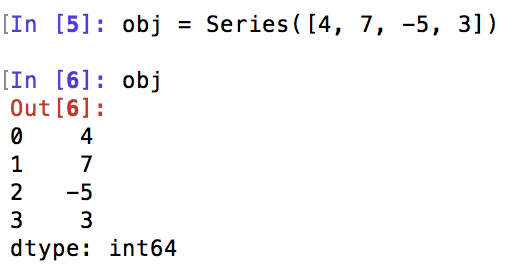
\includegraphics[width=.5\textwidth]{Cap4/imagens/pandas-series}}
	\caption{Exemplo de uma \textit{Series}}
	\vspace{-0.3cm}
	\legend{FONTE: \citeonline{python-analysis}}
	\label{pandas-series}
\end{figure}

\textit{DataFrame} representa uma tabela, uma estrutura de dados do tipo planilha, que possui uma coleção ordenada de colunas, onde cada uma delas pode ter um tipo de valor diferente (numérico, \textit{string}, \textit{boolean}, etc.). O \textit{DataFrame} possui um índice para linhas e também para colunas. Pode ser interpretado como um dicionário de \textit{Series}. De uma maneira geral, o dado é armazenado como um ou mais blocos bi-dimensionais ao invés de uma lista, dicionário, ou outro tipo de coleção de matriz unidimensional \cite{python-analysis}.

Existem várias maneiras diferentes de se criar um \textit{DataFrame}, entretanto uma forma comum é um dicionário de dimensões iguais, conforme a Figura~\ref{pandas-dataframe} e a Figura~\ref{pandas-dataframe2}, ou uma matriz \textit{NumPy}.

\begin{figure}[h!]
	\centering
	\fbox{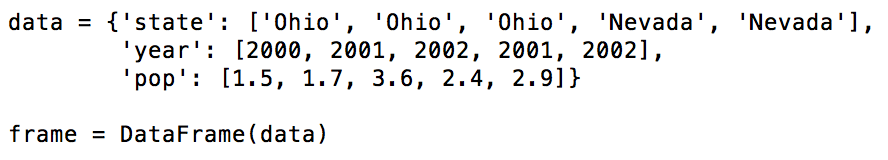
\includegraphics[width=.9\textwidth]{Cap4/imagens/pandas-dataframe}}
	\caption{Criação de um \textit{DataFrame}}
	\vspace{-0.3cm}
	\legend{FONTE: \citeonline{python-analysis}}
	\label{pandas-dataframe}
\end{figure}

\begin{figure}[h!]
	\centering
    \fbox{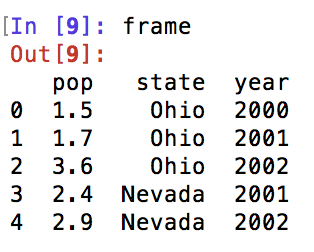
\includegraphics[width=.36\textwidth]{Cap4/imagens/pandas-dataframe2}}
	\caption{Conteúdo de um \textit{DataFrame} pelo interpretador \textit{IPython}}
	\vspace{-0.3cm}
	\legend{FONTE: \citeonline{python-analysis}}
	\label{pandas-dataframe2}
\end{figure}

%%% sub: matplotlib
\subsubsection{Biblioteca \textit{matplotlib}}
O pacote \textit{matplotlib} é desenvolvido para a geração de gráficos bidimensionais a partir de \textit{arrays}. Gráficos comuns podem ser criados com alta qualidade a partir de simples comandos, inspirados nos comandos gráficos do MATLAB, exemplo ilustrado na Figura~\ref{matplotlib-fig}.

Quando usado em conjunto com ferramentas GUI (\textit{IPython}, por exemplo), esta biblioteca possui recursos interativos como zoom e visão panorâmica. Além disto, suporta várias ferramentas GUI \textit{backend}, nos diversos sistemas operacionais suportados pelo Python, e permitem exportar gráficos em diversos formatos: PDF, SVG, JPG, PNG, BMP, GIF, etc.

\textit{matplotlib} também possui várias ferramentas adicionais, como o \textit{mplot3d} para plotar gráficos tridimensionais, e o \textit{basemap} para mapeamentos e projeções.

\begin{figure}[h!]
  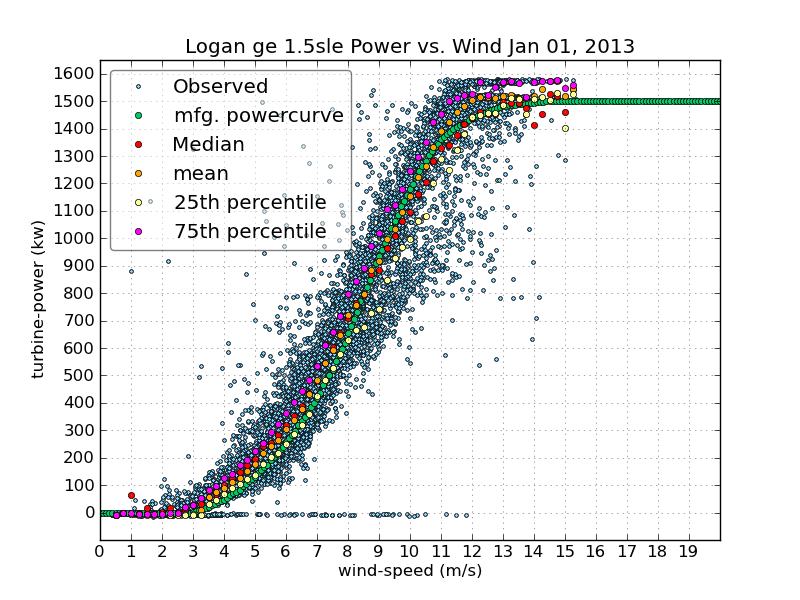
\includegraphics[width=1\textwidth]{Cap4/imagens/matplotlib}
  \caption{Exemplo de um gráfico gerado pelo \textit{matplotlib}}
  \vspace{-0.3cm}
  \legend{FONTE: \citeonline{matplotlib}}
  \label{matplotlib-fig}
\end{figure}


%%% sub: SciPy
\subsubsection{Biblioteca \textit{SciPy}}
\textit{SciPy} é uma coleção de pacotes que abordam uma série de soluções para diferentes domínios na computação científica. Na lista a seguir são apresentados exemplos desses pacotes \cite{python-analysis}:

\begin{itemize}
	\item \textit{scipy.integrate}: rotinas de integração numéricas e soluções de equações diferenciais;
	\item \textit{scipy.linalg}: rotinas de álgebra linear e decomposição de matrizes;
	\item \textit{scipy.optimize}: funções otimizadoras (minimizadoras) e algoritmos de busca em raíz;
	\item \textit{scipy.signal}: ferramentas para processamento de sinais;
	\item \textit{scipy.sparse}: matrizes esparsas e soluções de sistemas lineares esparsos;
	\item \textit{scipy.special}: agregador do \textit{SPECFUN}, uma biblioteca do Fortran que implementa várias funções matemáticas, como exemplo, a função gama;
	\item \textit{scipy.stats}: funções estatísticas, variáveis contínuas e discretas, testes estatísticos e outros modelos estatísticos;
	\item \textit{scipy.weave}: ferramenta para usar códigos \textit{inline} de C++ para acelerar a computação de matrizes.
\end{itemize}


%%% sub: IPython
\subsubsection{Interpretador \textit{IPython}}
O interpretador \textit{IPython} teve seu desenvolvimento iniciado em 2001, com o intuito de ser um interpretador interativo para a linguagem Python. Desde a sua criação o \textit{IPython} evoluiu grandemente, ao ponto de ser considerada uma das mais importantes ferramentas para computação científica em Python. Essa biblioteca não oferece nenhuma ferramenta para análise de dados ou análise computacional em si, sendo designada para maximizar a produtividade, tanto na interação computacional como no desenvolvimento de softwares. Oferece um fluxo de visualização de um modo \textit{execute-explore} ao invés do típico modelo \textit{edit-compile-run} de muitas outras linguagens de programação. Ela também provê uma pequena integração com o \textit{shell} e sistemas de arquivos. Como a maior parte da programação focada na mineração de dados envolve exploração, tentativa, erro e iteração, \textit{IPython}, em quase todos os casos, irá facilitar este tipo de trabalho \cite{python-analysis}.

Hoje, o projeto \textit{IPython} engloba muito mais do que apenas um interpretador \textit{shell} para Python. Ele também inclui um console gráfico interativo, o \textit{IPython Notebook}, que provê ao usuário uma experiência de caderno (\textit{notebook-like}) através de um navegador \textit{web}, conforme Figura~\ref{ipython-fig}, e dispõe de um mecanismo de processamento paralelo. Assim como muitas outras ferramentas desenvolvidas para programadores, é extremamente customizável \cite{mining-social-web}. \\ \\ \\ \\ \\ \\ \\

\begin{figure}[h!]
  \centering
  \fbox{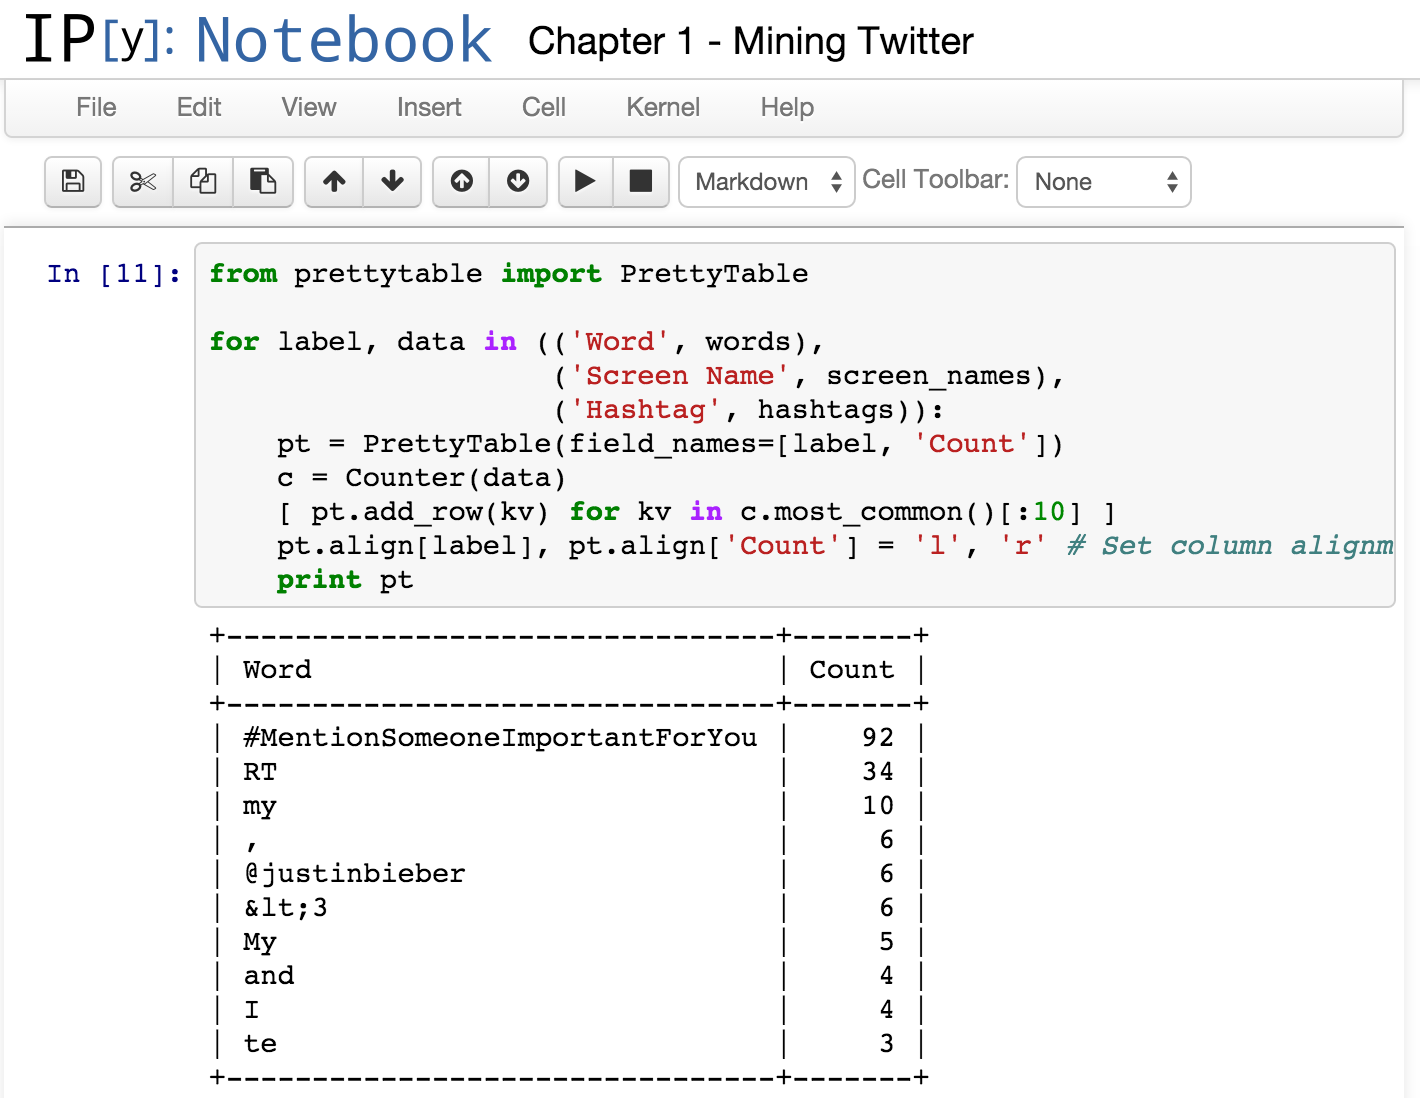
\includegraphics[width=0.9\textwidth]{Cap4/imagens/ipython-notebook}}
  \caption{Exemplo de uma página \textit{web} do \textit{IPython Notebook}}
  \vspace{-0.3cm}
  \legend{FONTE: \citeonline{python-analysis}}
  \label{ipython-fig}
\end{figure}

% python-linkedin
\subsubsection{Biblioteca \textit{python-linkedin}}
Esta biblioteca provê ao Python a API do \textit{LinkedIn}. Através da utilização do protocolo OAuth 2.0, é possível acessar diveros campos como \textit{Profile}, \textit{Group}, \textit{Company}, \textit{Jobs}, \textit{Search}, \textit{Share}, \textit{Network} e requisições REST APIs \cite{python-linkedin}.

%%
% API
\subsection{Interface de Programação de Aplicações - API}\label{subsec: api}
API é uma sigla para \textit{Application Programming Interface} e basicamente é uma tecnologia que permite um pedaço de \textit{software} se comunicar com outro pedaço de \textit{software}. Existem vários tipos de API e é comumente referenciado a outras tecnologias. Por exemplo, para o desenvolvimento deste trabalho será utilizado a API do \textit{LinkedIn}. 

Uma API é composta por uma série de funções acessíveis somente por programação, e que permitem utilizar características do \textit{software} menos evidentes ao utilizador tradicional.


%% 
% REST API
\subsubsection{Arquitetura REST}
Abreviação para Transferência de Estado Representacional (REST), é um estilo arquitetural baseado em recursos e nas representações desses recursos. Enfatiza a escalabilidade na interação entre componentes, a generalidade de interfaces, a implantação independente dos componentes de um sistema, o uso de componentes intermediários visando a redução na latência de interações, o reforço na segurança e o encapsulamento de sistemas legados. A REST ignora os detalhes da implementação de componente e a sintaxe de protocolo com o objetivo de focar nos papéis dos componentes, nas restrições sobre sua interação com outros componentes e na sua interpretação de elementos de dados significantes \cite{rest}.

REST foi um termo criado por \citeonline{rest}, onde ele modela um estilo de arquitetura para a construção de serviços \textit{web} consistentes e coesos. O estilo da arquitetura REST é baseado em recursos e nos estados desses recursos.

A funcionalidade de uma REST API é similar ao funcionamento de uma página \textit{web}, onde o usuário efetua uma requisição a um servidor \textit{web}, utilizando o protocolo HTTP, e recebe dados como resposta.

Um recurso é qualquer conteúdo ou informação que é exposto na Internet, podendo ser um documento, vídeo clip, até processos de negócio ou dispositivos. Para utilizar um recurso é necessário ser capaz de identificá-lo na rede e de ter meios para manipulá-lo. Tem-se então, o \textit{Uniform Resource Identifiers} (URI) para este propósito. Um URI unicamente identifica um recurso e, ao mesmo tempo, o torna endereçável ou capaz de ser manipulado utilizando um protocolo, como o HTTP. \textbf{\textcolor{red}{[QUE ISSO?][}}O URI de um recurso se distingue dos de qualquer outro recurso e é através do próprio URI que ocorrem as interações com o recurso \cite{rest-book}.\textbf{\textcolor{red}{]}}

Recursos devem possuir pelo menos um identificador para ser endereçável, e cada identificador é associado com uma ou mais representações, que é uma transformação ou uma visão do estado do recurso em um instante de tempo. Essa visão é codificada em um ou mais formatos transferíveis, tal como XHTML, Atom, texto simples, XML, YML, JSON, JPG, MP3, entre outros  \cite{rest-book}.

Os recursos provêm o conteúdo ou objeto com o qual se quer interagir e para atuar sobre eles é utilizado os métodos de HTTP. Os métodos HTTP na arquitetura REST podem ser referenciados como Verbos, uma vez que representam ações sobre os recursos \cite{rest-book}.


\subsection{Protocolo de Autenticação - OAuth}
\textbf{\textcolor{red}{[MELHORAR]}} Protocolos de autenticação são capazes de, simplesmente, autenticar a parte que está se conectando, ou ainda de autenticar a parte que está conectando, assim como se autenticar para ele.

Neste trabalho será utilizado apenas o protocolo OAuth 2.0 para o acesso aos dados do \textit{LinkedIn}. É possível também, realizar a autenticação utilizando a versão mais antiga, OAuth 1.0a, mas será apenas referenciado, neste trabalho, para a melhor compreensão do funcionamento do protocolo.

OAuth é uma sigla para "\textit{open authorization}", ou autorização aberta, e provê um meio para que usuários autorizem uma aplicação acessar dados, com alguma finalidade, através de uma API, sem que os usuários precisem passar credenciais como nome de usuário e senha. De um modo geral, usuários são capazes de controlar o nível de acesso para estas aplicações e revogar este controle a qualquer momento \cite{mining-social-web}.

\subsubsection{Protocolo OAuth 1.0a}
OAuth 1.0a é um protocolo que permite que um cliente (\textit{client}) \textit{web} tenha acesso a um recurso protegido pelo seu dono em um servidor. Esta definição se dá através da RFC 5849. Que são documentos técnicos desenvolvidos e mantidos pelo Internet Enginnering Task Force (IETF), instituição que especifica os padrões que serão implementados e utilizados em toda a Internet.

A razão para a existência dessa tecnologia é para evitar problemas de usuários (donos dos recursos) compartilhar suas senhas com aplicações \textit{web}.

A versão OAuth 1.0a não permite que credenciais sejam trocadas utilizando uma conexão \textit{Secure Socket Layer} (SSL) através de um protocolo HTTPS. Por esse motivo, muitos desenvolvedores achavam tedioso o trabalho devido aos vários detalhes envolvidos em encriptação.

SSL é um padrão global para tecnologia de segurança. Tem como função principal criar um canal criptografado entre um servidor \textit{web} e um navegador (\textit{browser}) para garantir que todos os dados transmitidos sejam seguros e sigilosos.

Uma aplicação que está requerindo acesso é conhecida como \textit{client}, em alguns momentos chamado de \textit{consumer}, a rede social ou o serviço que contém os recursos protegidas é nomeado como \textit{server} (também chamado de \textit{provider}) e o usuário que concede o acesso é o \textit{resource owner} (dono do recurso, tradução livre). Com estes elementos, as três participações que envolvem o processo e a interação que estes elementos possuem é conhecida como \textit{"three-legged-flow"} ou de uma maneira mais coloquial, a \textit{OAuth dance}. Estas são as etapas fundamentais que envolvem a \textit{OAuth dance} que, como resultado, permite ao \textit{client} o acesso a recursos protegidos, conforme listado a seguir \cite{mining-social-web}:

\begin{enumerate}
	\item O \textit{client} obtém um \textit{token} de requisição do servidor de serviço (aplicação);
	\item O dono do recurso autoriza o \textit{token} de requisição;
	\item O \textit{client} troca o \textit{token} de requisição por um \textit{token} de acesso;
	\item O \textit{client} usa o \textit{token} de acesso para acessar os recursos protegidos com a consideração do dono do recurso.
\end{enumerate}

Para credenciais particulares, um \textit{client} começa com uma \textit{consumer key} e um \textit{consumer secret} e no fim do processo de \textit{OAuth dance}, termina com um \textit{token} de acesso e \textit{token} de acesso secreto que pode ser usado para acessar recursos protegidos.

\subsubsection{Protocolo OAuth 2.0}
Enquanto o protocolo OAuth 1.0a permite uma autorização útil para o acesso a aplicações \textit{web}, o OAuth 2.0 foi originalmente destinado a simplificar, significantemente, a implementação detalhada para desenvolvedores de aplicações \textit{web}, baseando-se completamente no SSL para aspectos de segurança e para satisfazer uma vasta quantidade de casos de uso. Esses casos de uso variaram desde suporte para dispositivos móveis à necessidades empresariais e, consequentemente, às necessidades de um termo mais futuro, da "Internet das Coisas"\space \cite{mining-social-web}.

Diferentemente da implementação OAuth 1.0a, que consiste de um rígido conjunto de etapas, a implementação do OAuth 2.0, definido através do RFC 6749, pode variar de acordo com a particularidade do caso de uso. Um decorrer típico da execução do OAuth 2.0 tem a vantagem do SSL e, essencialmente, contém apenas poucos redirecionamentos que,\textbf{\textcolor{red}{[}} acompanhada de em alto-nível, \textbf{\textcolor{red}{][QUE ISSO?]}}não possui tanta diferença em relação ao processo anterior que envolvem um ciclo do OAuth 1.0a.

%%
% Linkedin
\subsection{Rede Social LinkedIn}
\textit{LinkedIn} é uma rede social diferenciada, pois é voltada para perfis profissionais. Os usuários geralmente utilizam a rede como um currículo \textit{online}, procuram se relacionar com novos contatos para aumentar a sua rede de conhecimentos profissionais e, também, para encontrar e conhecer novas oportunidades, tanto de ocupação quanto de negócio.

A mineração de dados através da rede \textit{LinkedIn} se dá utilizando a API que ela dispõe. Para isso, é necessário possuir uma conta nesta rede social.

A grande parte das análise realizadas neste projeto acontece utilizando arquivos \textit{comma-separated values} (CSV) \textbf{\textcolor{red}{[BREEVE DEFINIÇÃO]}}, que podem ser baixados.

Na Subseção~\ref{api-linkedin} é apresentado a API do \textit{LinkedIn} e como se obter dados através dela.

\subsubsection{API LinkedIn \textbf{\textcolor{red}{[MAIS DETALHES SOBRE API - MELHORAR]}}}\label{api-linkedin}
O acesso a API se dá através da criação de uma aplicação pela página \textit{web} de desenvolvimento do \textit{LinkedIn}. Após a criação da aplicação é fornecido ao usuário informações para o acesso utilizando o protocolo OAuth, será informado uma chave da API da aplicação, uma chave secreta, o \textit{token} de usuário OAuth e credenciais secretas do usuário OAuth.

Dispondo de todas as credenciais do protocolo OAuth o acesso à API acontece utilizando a biblioteca \textit{python-linkedin}, especificada na subseção~\ref{sec:bib_python}.

Os dados disponibilizados pela API estão limitados, basicamente, ao o que o usuário consegue usufruir da sua experiência através da página \textit{web}. Restrições como a visualização de "amigos de amigos" \space também existem, demonstrando ser uma API um tanto restrita. Essa restrição é proposital e importante para a política do \textit{LinkedIn}. Portanto, é possível fazer buscas de pessoas, companhias, empregos, conexões, grupos e outros elementos que a API disponibiliza \cite{mining-social-web}.

Conforme descrito anteriormente, é possível fazer o \textit{download} dos dados, visíveis ao usuário, em formato CSV, podendo ser especificados em títulos de trabalho ou contatos através de uma opção de exportação presente no menu da página do \textit{LinkedIn}.

%%
% METODOLOGIA
\section{METODOLOGIA E DESENVOLVIMENTO \textbf{\textcolor{red}{[REFAZER]}}}\label{sec: metodologia}
O processo de desenvolvimento da solução segue uma série de princípios de conjunto de boas práticas e etapas do \textit{data mining}, para melhor estruturar e obter, não só o resultado esperado, mas também para que todo o processo ocorra de forma coerente e padronizada.

%%
% Etapas do Data Mining
\subsection{Etapas Para a Mineração de Dados do \textit{LinkedIn}}
Abordado previamente, o acesso aos dados do \textit{LinkedIn} acontece através da utilização de sua API e a interpretação dos dados se dá pela aplicação da técnica de \textit{clustering}, normalização de dados e computação de similaridade. 

\subsubsection{\textit{Clustering}}
A técnica de \textit{clustering} é um aprendizado não supervisionado que está presente em várias ferramentas de \textit{data mining}. Consiste na adoção de uma coleção de itens e, após particioná-los em pequenas coleções, conhecidos como \textit{cluster}, baseando-se em alguma heurística que será usada para comparar com outros itens da coleção.

\textbf{\textcolor{red}{[ESTUDAR MAIS ATÉ O FINAL]}}

Técnicas para \textit{clustering} são partes fundamentais para um processo de mineração de dados. Uma implementação simples de \textit{clustering} pode criar experiências de usuário incrivelmente convincentes para alcançar resultados. Também pode ser aplicado a bases de texto utilizando algoritmos de \textit{text mining}, onde o algoritmo procura agrupar textos que falem sobre o mesmo assunto e separar textos de conteúdo diferentes.

Por exemplo, caso queira considerar a localização geográfica dos contatos na rede \textit{LinkedIn}, é necessário realizar um \textit{cluster} nas conexões através de um determinado número de regiões com o intuito da melhor compreensão de oportunidades econômicas disponíveis.

\subsubsection{Normalização de Dados}
Quando se recupera dados provenientes de uma API, é muito comum que esses não estarão no formato desejado para a sua análise. No caso do \textit{LinkedIn}, pode ser que usuários procurem por vagas de emprego escrevendo os nomes das vagas de alguma outra maneira sem ser o nome correto da vaga. Como exemplo, uma vaga para administrador de banco de dados pode ser buscado através da sigla "DBA", que em inglês significa \textit{Database Administrator}.

A normalização de dados, procura então resolver esses problemas padronizando situações específicas que irá facilitar a análise posterior dos dados.

\subsubsection{Computação de Similaridade}
Após a normalização dos itens, é preciso verificar a similaridade entre eles. Podendo ser vagas de emprego, nomes de empresas, interesses profissionais, indicação geográfica, ou qualquer outro campo digitado na busca como um texto livre. Para isso é necessário definir uma heurística que conseguirá aproximar a similaridade entre dois valores quaisquer. Em algumas situações a similaridade heurística será um tanto óbvia, porém em outros casos será complicada. Por exemplo, comparar o tempo de carreira entre duas pessoas pode ser simples como uma operação de soma ou subtração. Mas comparar um elemento profissional, como "atitude de liderança" \space de uma maneira automatizada pode ser um desafio.



















